\documentclass[journal,12pt,onecolumn]{IEEEtran}
\usepackage{cite}
\usepackage{caption}
\usepackage{graphicx}
\usepackage{amsmath,amssymb,amsfonts,amsthm}
\usepackage{algorithmic}
\usepackage{graphicx}
\usepackage{textcomp}
\usepackage{xcolor}
\usepackage{tfrupee}
\usepackage{txfonts}
\usepackage{listings}
\usepackage{enumitem}
\usepackage{mathtools}
\usepackage{gensymb}
\usepackage{comment}
\usepackage[breaklinks=true]{hyperref}
\usepackage{tkz-euclide} 
\usepackage{listings}
\usepackage{gvv}
%\def\inputGnumericTable{}
\usepackage[latin1]{inputenc} 
\usetikzlibrary{arrows.meta, positioning}
\usepackage{xparse}
\usepackage{color}                                            
\usepackage{array}                                            
\usepackage{longtable}                                       
\usepackage{calc}                                             
\usepackage{multirow}
\usepackage{multicol}
\usepackage{hhline}                                           
\usepackage{ifthen}                                           
\usepackage{lscape}
\usepackage{tabularx}
\usepackage{array}
\usepackage{float}
\usepackage{marvosym}
\usepackage{float}
%\newcommand{\define}{\stackrel{\triangle}{=}}
\theoremstyle{remark}
\usepackage{circuitikz}
\captionsetup{justification=centering}
\usepackage{tikz}

\title{Matrices in Geometry 5.8.35}
\author{EE25BTECH11037 - Divyansh}
\begin{document}
\vspace{3cm}
\maketitle
{\let\newpage\relax\maketitle}
\textbf{Question: }
The cost of $4 \ kg$ onion, $3 \ kg$ wheat and $2\ kg$ rice is \rupee $60$. The cost of $2 \ kg$ onion, $4 \ kg$ wheat, and $6 \ kg$ rice is \rupee $90$. The cost of $6 \ kg$ onion, $2\ kg$ wheat, and $3\ kg$ rice is \rupee $70$. Find the cost of each item per kilogram.
 
\vspace{2mm}


\textbf{Solution:}
\\
Let the cost of 1 kg of onion, wheat and rice be \rupee $x$, \rupee $y$ and \rupee $z$, respectively.

The given information is:
\begin{align}
    \myvec{4 & 3 & 2}\myvec{x \\ y \\ z}=60 \\
    \myvec{2 & 4 & 6}\myvec{x \\ y \\ z}=90 \\
    \myvec{6 & 2 & 3}\myvec{x \\ y \\ z}=70 
\end{align}
Stacking them in a single matrix:
\begin{align}
    \myvec{4 & 3 & 2 \\ 2 &  4& 4 \\ 6 & 2 & 3}\myvec{x \\ y \\ z}=\myvec{60 \\ 90 \\ 70}
\end{align}
Writing the augmented matrix
\begin{align}
    \myvec{4 & 3 & 2 & \vrule & 60 \\ 2 &  4& 6 & \vrule & 90\\ 6 & 2 & 3& \vrule & 70}
    \overset{R_1 \rightarrow R_1 /4, R_2 \rightarrow R_2/2}{\longleftrightarrow}
    \myvec{1 & 3/4 & 1/2 & \vrule & 15 \\ 1 &  2& 3 & \vrule & 45\\ 6 & 2 & 3& \vrule & 70}
    \overset{R_2\rightarrow R_2-R_1, R_3 \rightarrow R_3 - 6R_1}{\longleftrightarrow}\\
    \myvec{1 & 3/4 & 1/2 & \vrule & 15 \\ 0 &  5/4& 5/2 & \vrule & 30\\ 0 & -5/2 & 0& \vrule & -20}\overset{R_2 \rightarrow 4R_2/5}{\longleftrightarrow}
    \myvec{1 & 3/4 & 1/2 & \vrule & 15 \\ 0 &  1& 2 & \vrule & 24\\ 0 & -5/2 & 0& \vrule & -20} \overset{R_1 \rightarrow R_1 - 3R_2/4, R_3 \rightarrow R_3 + 5R_2/2}{\longleftrightarrow}\\
    \myvec{1 & 0 & -1 & \vrule & -3 \\ 0 &  1& 2 & \vrule & 24\\ 0 & 0 & 5& \vrule & 40}
    \overset{R_3 \rightarrow R_3/5}{\longleftrightarrow}\myvec{1 & 0 & -1 & \vrule & -3 \\ 0 &  1& 2 & \vrule & 24\\ 0 & 0 & 1& \vrule & 8} \overset{R_1 \rightarrow R_1 + R_3, R_2 \rightarrow R_2 - 2R_3}{\longleftrightarrow}\myvec{1 & 0 & 0 & \vrule & 5 \\ 0 &  1& 0 & \vrule & 8\\ 0 & 0 & 1& \vrule & 8}
\end{align}

This implies that 
\begin{align}
    \myvec{x \\ y\\ z}=\myvec{5 \\ 8 \\ 8}
\end{align}
Therefore, the cost of 1 kg of onion, wheat, rice is \rupee $5$, \rupee $8$ and \rupee $8$.
\begin{figure}[H]
    \centering
    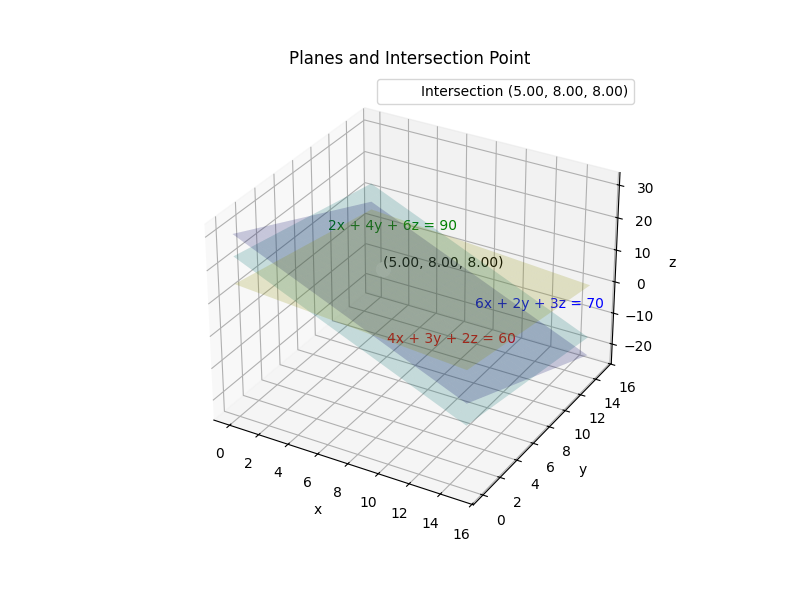
\includegraphics[width=1\columnwidth]{figs/1.png}
    \caption{Graph for 5.8.35}
    \label{fig:placeholder}
\end{figure}
\end{document}
